\section{LLM 服务与调度}
\label{sec:bg}

\subsection{背景：在集群中调度 LLM 请求}
\label{sec:llm-scheduling}

\begin{figure}[!t]
        \vspace{2mm}
        \begin{minipage}{1\linewidth}
        \centering
        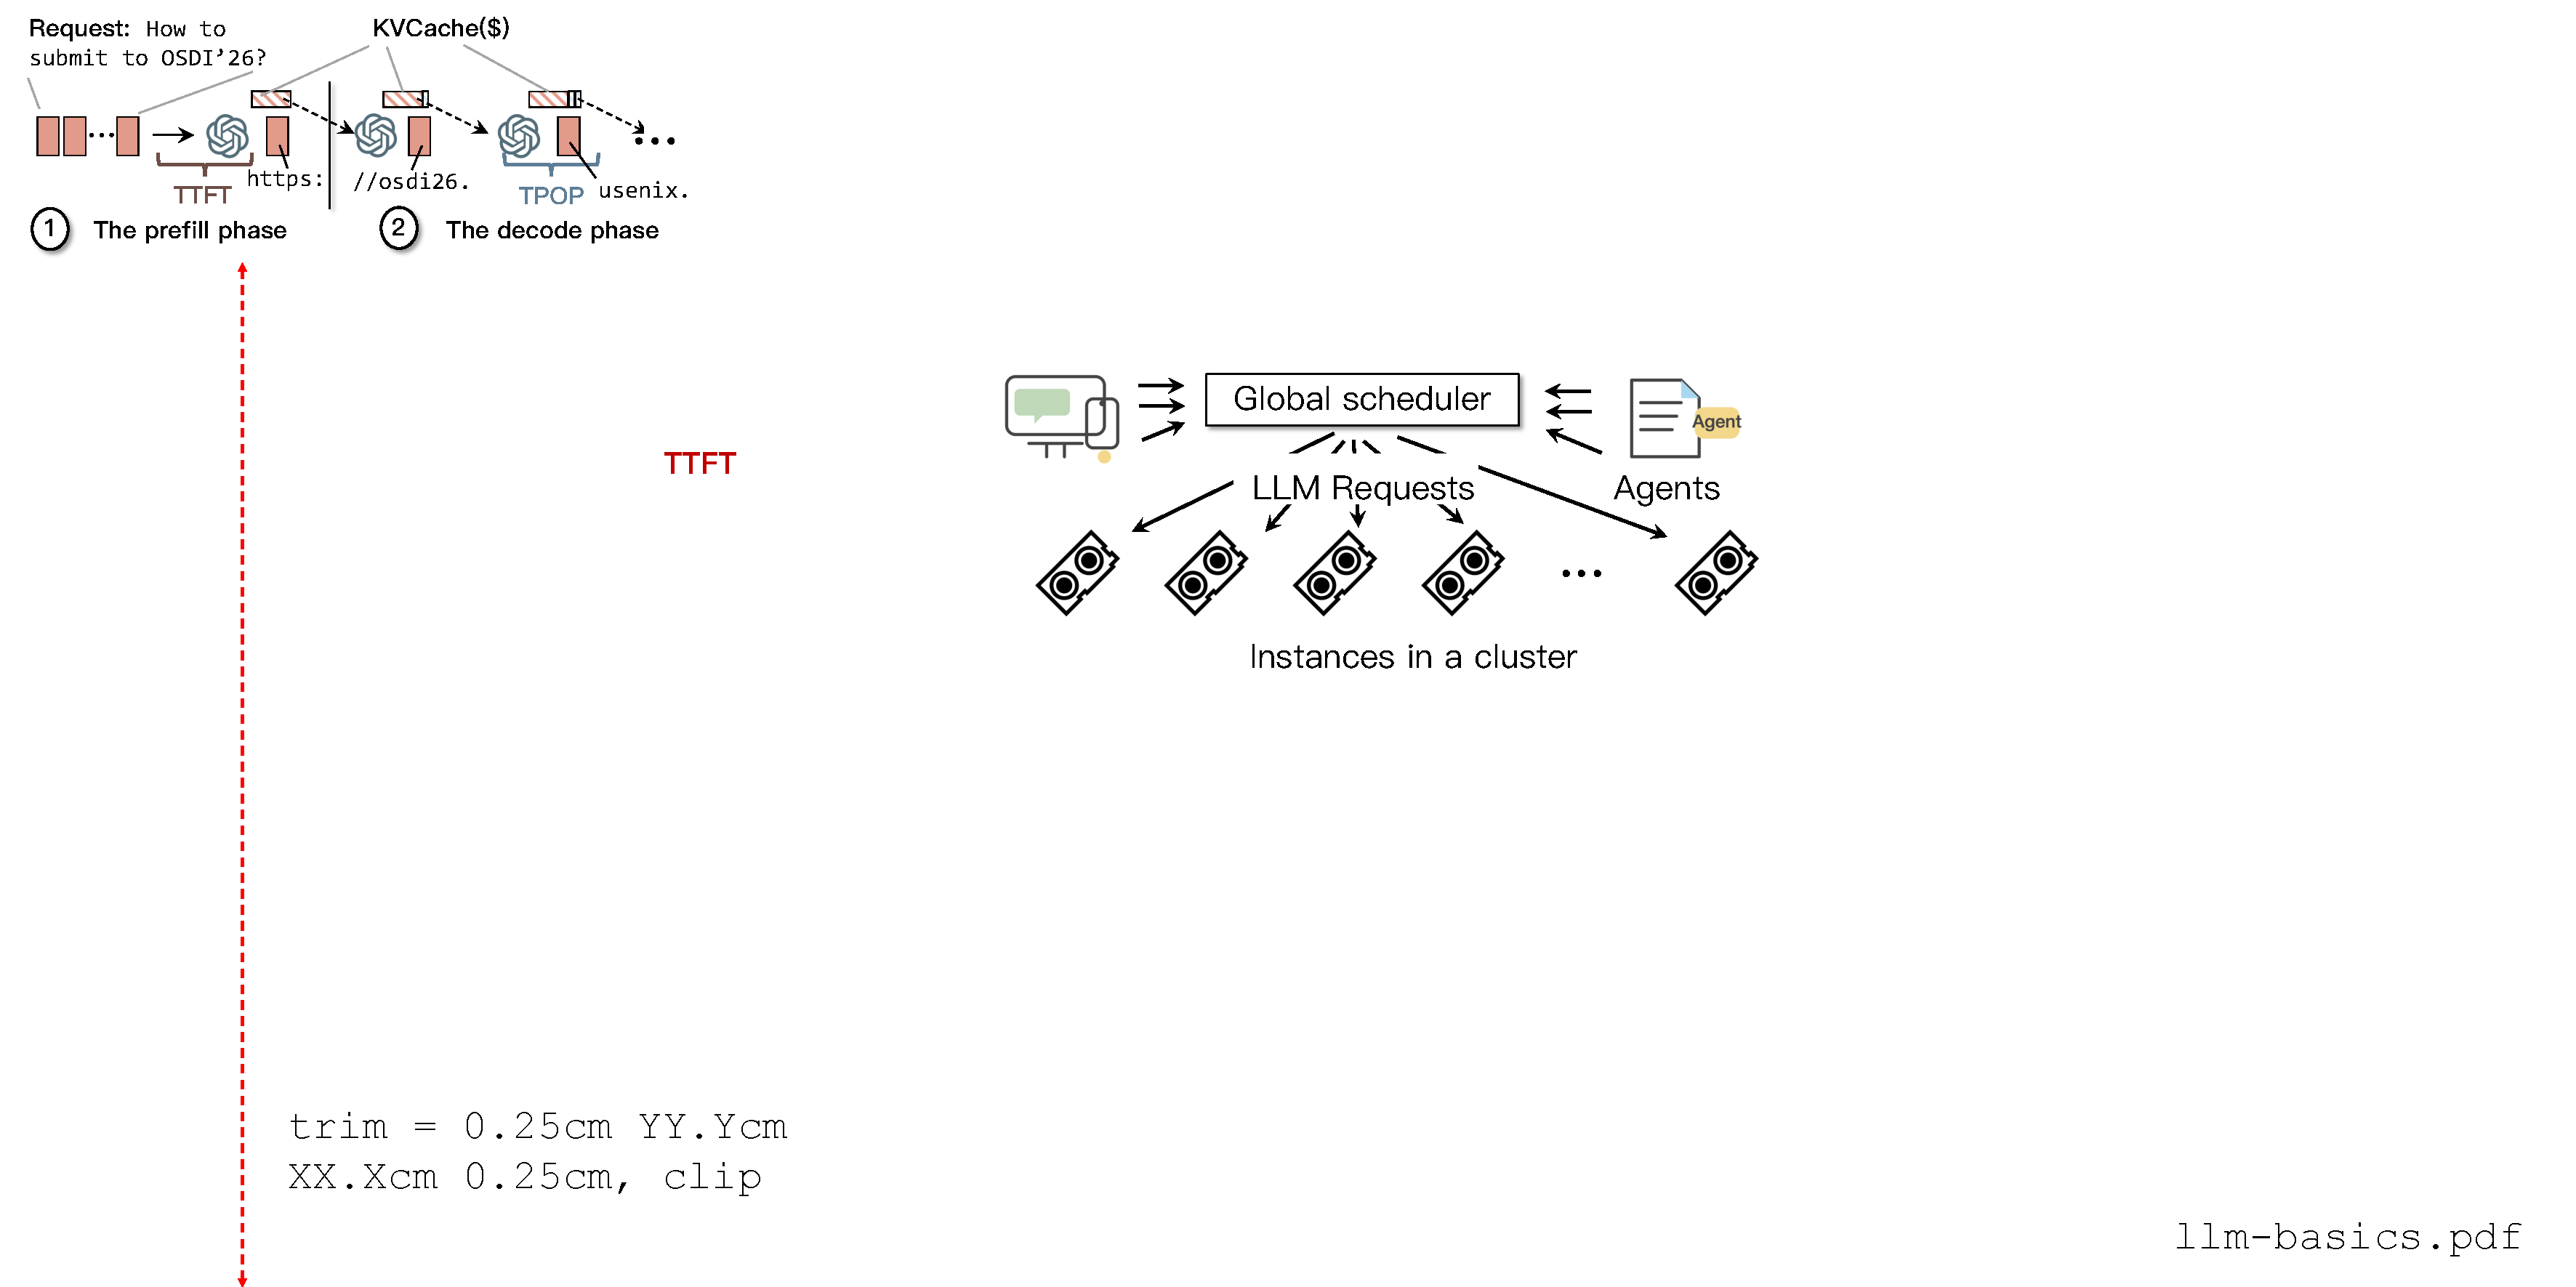
\includegraphics[width=0.95\linewidth, trim=0.25cm 23.92cm 43cm 0.25cm, clip]{figs/llm-basics.pdf}
        \end{minipage} \\[2pt]
        \begin{minipage}{1\linewidth}
        \caption{\small{%
            使用 LLM 生成输出 token 的示意图，以及两个性能指标：
            首 token 时间（TTFT）和每输出 token 时间（TPOT）。
        }}
        \label{fig:llm-basics}
        \end{minipage} \\[-0pt]
        \end{figure}


\nospacestitle{使用 LLM 处理请求（{\fig{fig:llm-basics}}）。\,}
LLM 以自回归方式生成 token，整个过程分为两个步骤：
\ding{192}：在\emph{预填充}阶段，输入 token 被送入模型，模型处理这些 token 并生成第一个输出 token。
之后，LLM 进入\emph{解码}阶段（\ding{193}），逐个生成后续 token。
每次生成都需要所有已生成 token 以及输入 token 的上下文。
为了加速生成，这些\emph{已处理上下文}会以张量形式物化并存储在 GPU 显存中，通常称为\emph{键值缓存}（{\kvcache}）。
因此，解码阶段的计算量显著小于预填充阶段，因为无需再为输入 token 生成 {\kvcache}。

从 LLM 服务提供商的角度看，与服务质量相关的两个关键性能指标是：
\emph{首 token 时间（TTFT）}和\emph{每输出 token 时间（TPOT）}。
TTFT 很重要，因为它直接决定了 LLM 服务对用户请求的响应速度；
而 TPOT 不仅影响后续交互的流畅度，也影响整个请求完成所需的总时间。

\begin{figure}[!t]
        \hspace{3mm}
        \begin{minipage}{1\linewidth}
%        \centering
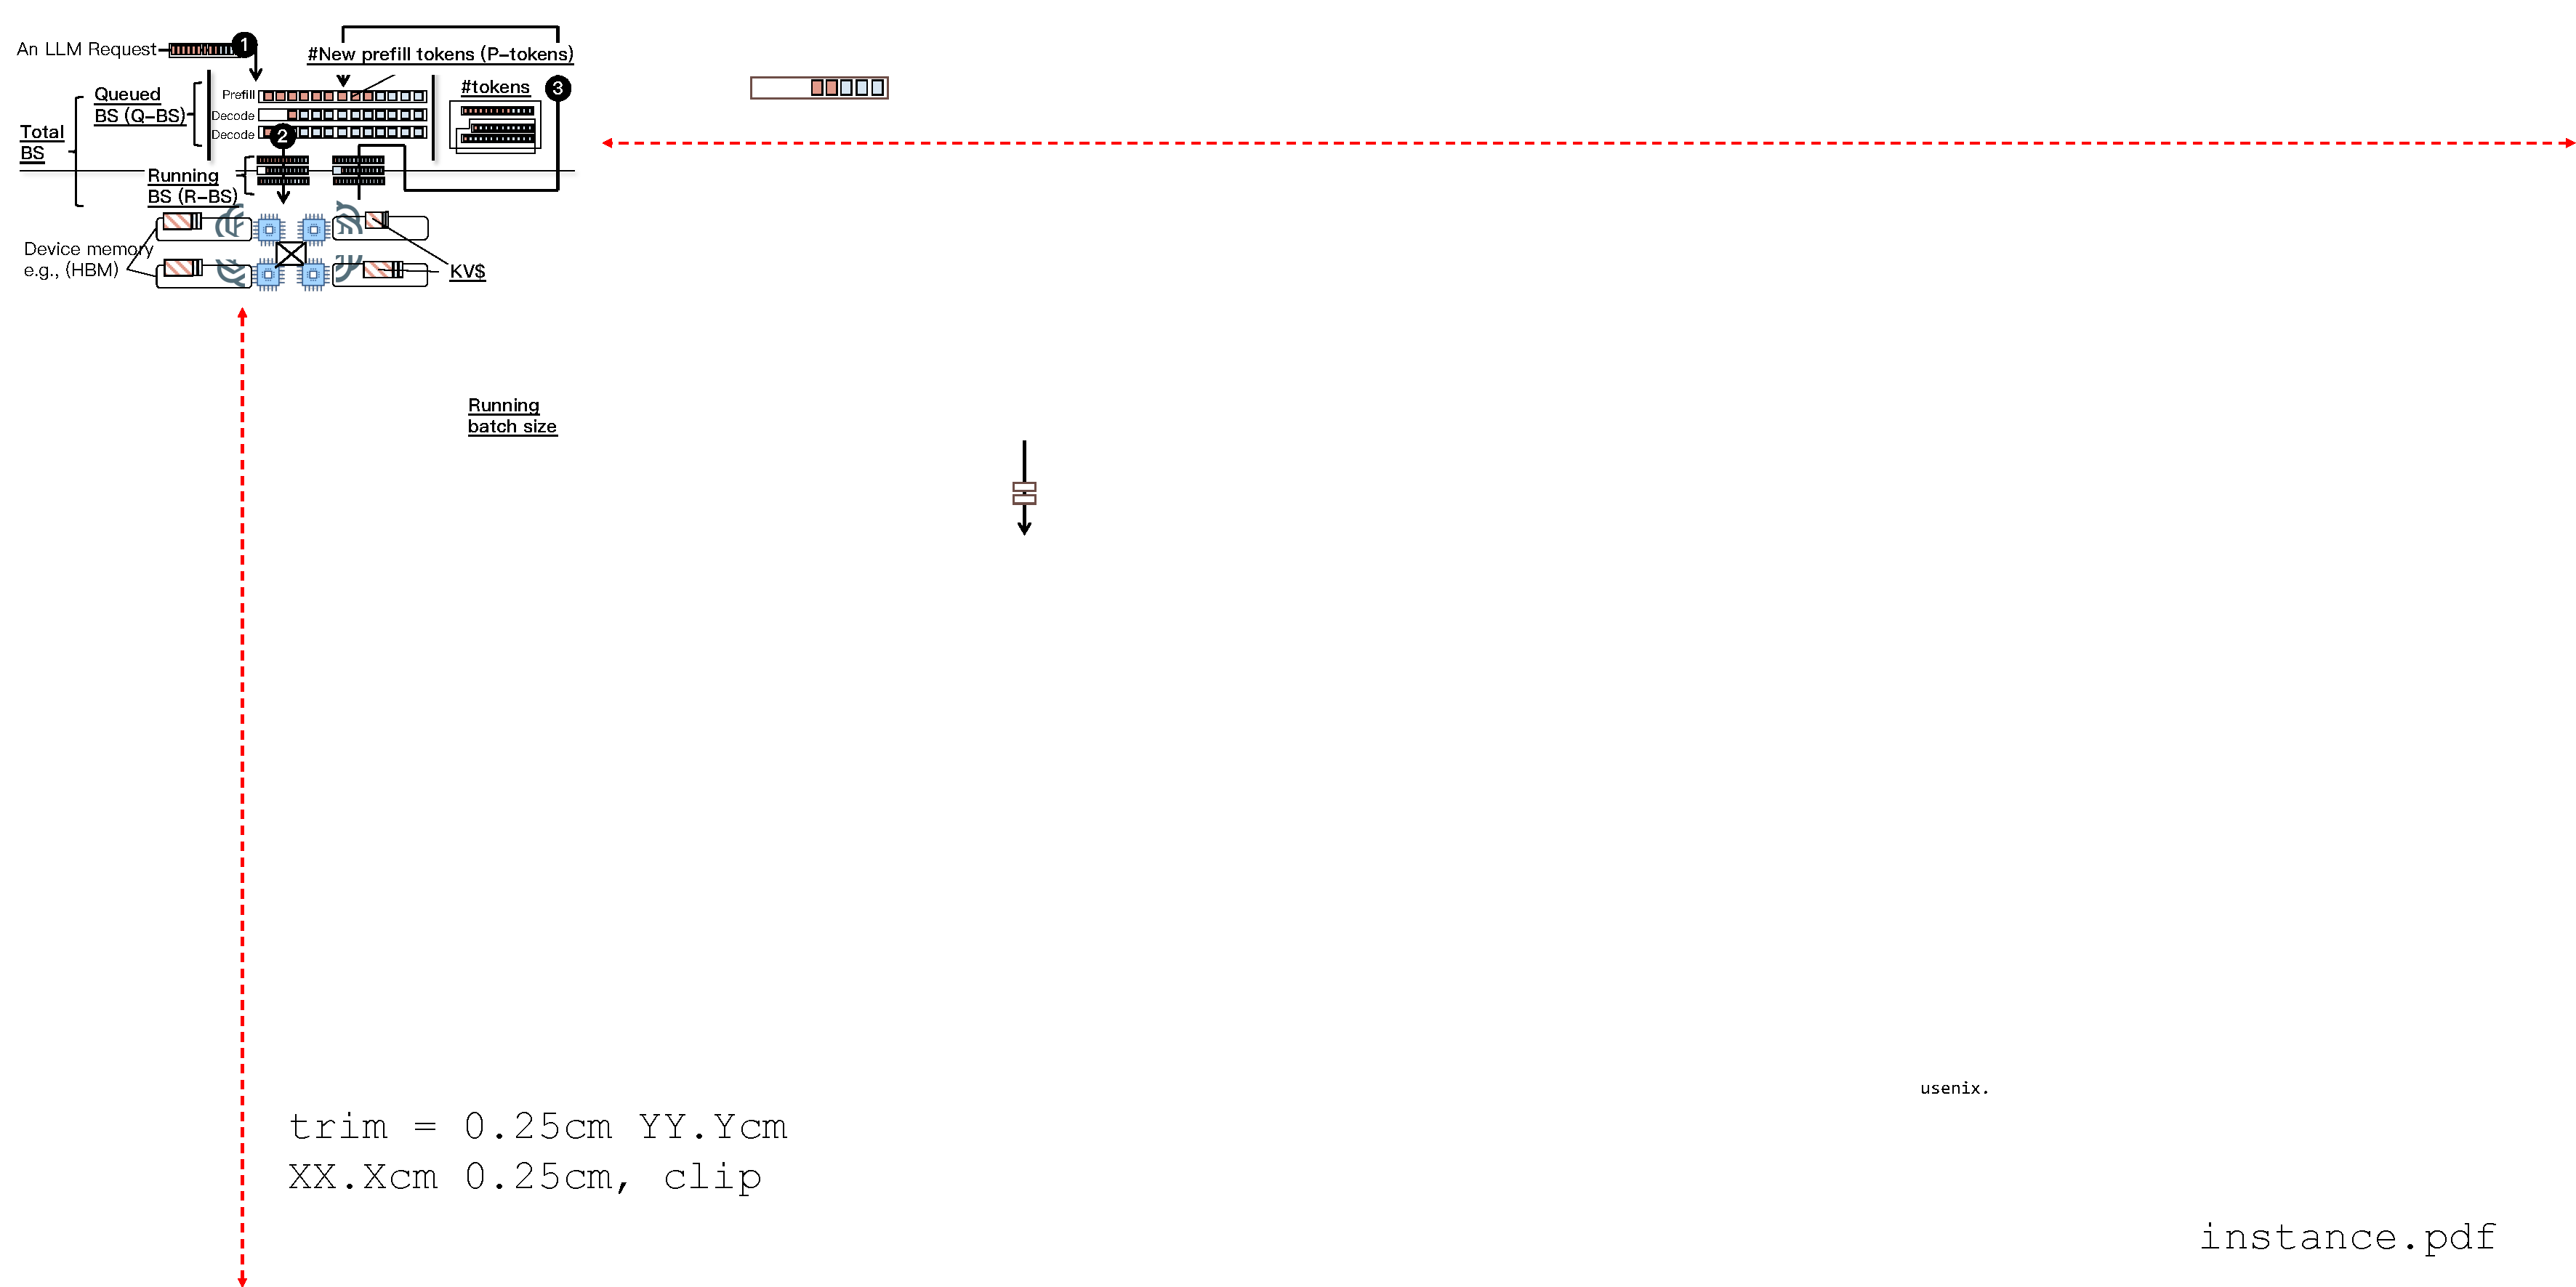
\includegraphics[width=0.92\linewidth, trim=0.25cm 22.9cm 46cm 0.25cm, clip]{figs/instance.pdf}
        \end{minipage} \\[4pt]
        \begin{minipage}{1\linewidth}
        \caption{\small{%
            LLM 服务实例如何处理请求的系统视图，以及全局调度器可以直接采集的一些系统\metric{指标}。
            每个指标的详细含义会在首次使用时说明。
            \textbf{BS} 是 \uline{b}atch \uline{s}ize（批大小）的缩写。
        }}
        \label{fig:llm-instance}
        \end{minipage} \\[5pt]
        \end{figure}


\stitle{服务实例与 {\kvcache} 缓存（{\fig{fig:llm-instance}}）。\,}
在 LLM 服务系统中，实例是处理请求的最小单元，并承载一份完整的 LLM 参数副本。
如果模型太大而无法装入单张 GPU 显存，一个实例也可以由多张 GPU 组成。
无论实例由单 GPU 还是多 GPU 构成，整体服务流程都是相同的：
当实例接收到请求后，请求会被压入该实例的队列中，队列里存放着等待在该实例上执行的请求（预填充或解码，\ding{182}）。
当 GPU 可用时，所有排队请求会被组成一个\emph{批次}，并结合 \emph{chunked prefill}~\cite{298679} 在 GPU 上高效执行（\ding{183}）。
执行完成后，实例会检查当前请求是否还需要进一步解码；如果需要，请求会被重新入队（\ding{184}）。

一个值得注意的特点是，该服务是\emph{有状态}的：即使请求已经完成生成，其 {\kvcache} 仍会保留在 GPU 或 CPU 内存中（即 {\kvcache} cache~\cite{305212,298501,10.5555/3768039.3768067}）。
这样做的好处在于，如果未来某个请求被路由到某实例，并且它与此前缓存的 {\kvcache} 存在前缀匹配，那么该实例就可以跳过对匹配前缀 token 的计算，从而显著降低计算成本。
在 {\fig{fig:llm-instance}} 的示例中，蓝色标出的 token 若发生 {\kvcache} 命中，就可以跳过对应计算。

\begin{figure}[!t]
%        \hspace{-2mm}
        \begin{minipage}{1\linewidth}
        \centering
        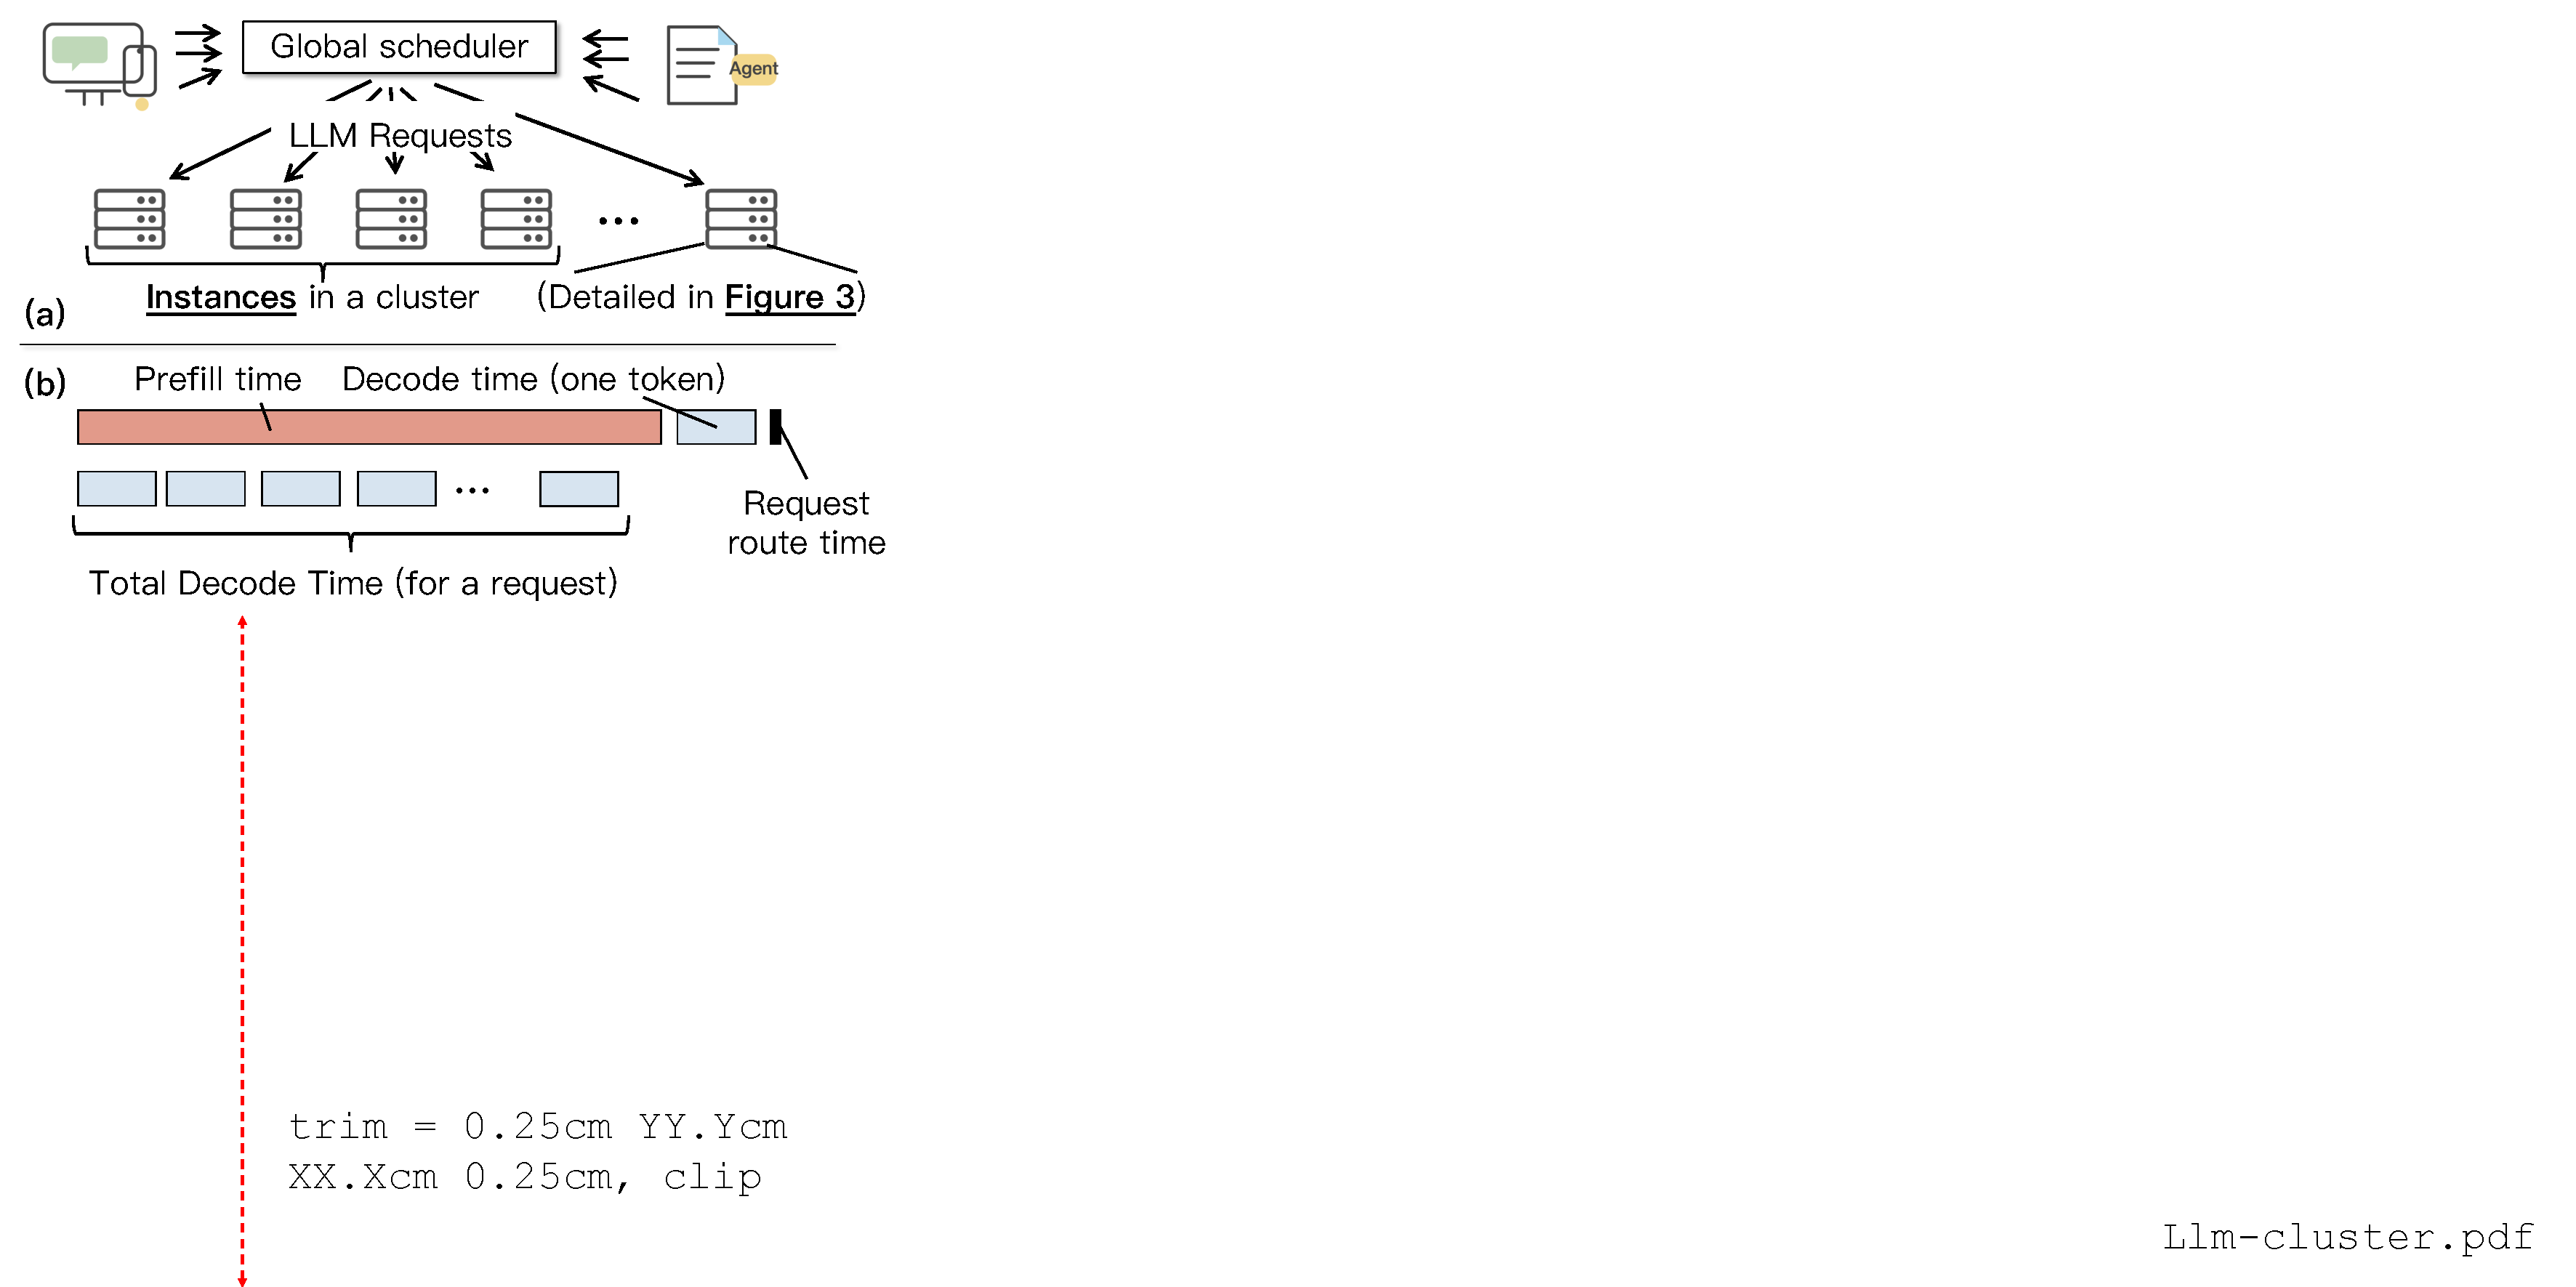
\includegraphics[width=0.85\linewidth, trim=0.25cm 15.7cm 39.65cm 0.25cm, clip]{figs/llm-cluster.pdf}
        \end{minipage} \\[4pt]
        \begin{minipage}{1\linewidth}
        \caption{\small{%
        (a) 集群式 LLM 服务系统的系统视图；
        以及
        (b) 单个请求的服务时间与路由开销的对比。
        }}
        \label{fig:setup}
        \end{minipage} \\[-10pt]
        \end{figure}

\stitle{集群中的请求调度（{\fig{fig:setup}}）。\,}
为了处理大量请求，LLM 服务提供商通常会部署由多个实例组成的模型服务集群。
每个集群都配有专门的\emph{全局调度器}，负责将请求路由到其管理的实例上，如图 (a) 所示。
调度器通过执行某种\emph{调度策略}来决定每个请求的目标实例，而这正是本文关注的重点。
需要注意的是，服务提供商也可能为同一个模型部署多个集群，以增强可靠性与地理亲和性；
而跨集群路由不在本文讨论范围内。

从高层看，现有所有调度策略都可以视为一个三步过程：
调度器首先（可选地）\emph{过滤}掉部分实例，随后按照某种偏好顺序对实例进行\emph{打分}，最后将请求路由到得分最优的实例。
这个分数建立在从各实例采集到的指标之上，我们将在后续分析中详细介绍这些指标（\textsection{\ref{sec:principles}}）。
